%% Copernicus Publications Manuscript Preparation Template for LaTeX Submissions
%% ---------------------------------
%% This template should be used for copernicus.cls
%% The class file and some style files are bundled in the Copernicus Latex Package, which can be downloaded from the different journal webpages.
%% For further assistance please contact Copernicus Publications at: production@copernicus.org
%% https://publications.copernicus.org/for_authors/manuscript_preparation.html


%% Please use the following documentclass and journal abbreviations for preprints and final revised papers.

%% 2-column papers and preprints
\documentclass[journal abbreviation, manuscript]{copernicus}



%% Journal abbreviations (please use the same for preprints and final revised papers)


% Advances in Geosciences (adgeo)
% Advances in Radio Science (ars)
% Advances in Science and Research (asr)
% Advances in Statistical Climatology, Meteorology and Oceanography (ascmo)
% Annales Geophysicae (angeo)
% Archives Animal Breeding (aab)
% ASTRA Proceedings (ap)
% Atmospheric Chemistry and Physics (acp)
% Atmospheric Measurement Techniques (amt)
% Biogeosciences (bg)
% Climate of the Past (cp)
% DEUQUA Special Publications (deuquasp)
% Drinking Water Engineering and Science (dwes)
% Earth Surface Dynamics (esurf)
% Earth System Dynamics (esd)
% Earth System Science Data (essd)
% E&G Quaternary Science Journal (egqsj)
% European Journal of Mineralogy (ejm)
% Fossil Record (fr)
% Geochronology (gchron)
% Geographica Helvetica (gh)
% Geoscience Communication (gc)
% Geoscientific Instrumentation, Methods and Data Systems (gi)
% Geoscientific Model Development (gmd)
% History of Geo- and Space Sciences (hgss)
% Hydrology and Earth System Sciences (hess)
% Journal of Bone and Joint Infection (jbji)
% Journal of Micropalaeontology (jm)
% Journal of Sensors and Sensor Systems (jsss)
% Magnetic Resonance (mr)
% Mechanical Sciences (ms)
% Natural Hazards and Earth System Sciences (nhess)
% Nonlinear Processes in Geophysics (npg)
% Ocean Science (os)
% Polarforschung - Journal of the German Society for Polar Research (polf)
% Primate Biology (pb)
% Proceedings of the International Association of Hydrological Sciences (piahs)
% Scientific Drilling (sd)
% SOIL (soil)
% Solid Earth (se)
% The Cryosphere (tc)
% Weather and Climate Dynamics (wcd)
% Web Ecology (we)
% Wind Energy Science (wes)


%% \usepackage commands included in the copernicus.cls:
%\usepackage[german, english]{babel}
%\usepackage{tabularx}
%\usepackage{cancel}
%\usepackage{multirow}
%\usepackage{supertabular}
%\usepackage{algorithmic}
%\usepackage{algorithm}
%\usepackage{amsthm}
%\usepackage{float}
%\usepackage{subfig}
%\usepackage{rotating}


\begin{document}

\title{Phydra v1 - an open-source toolbox for flexible and reproducible marine ecosystem modeling in Python}


% \Author[affil]{given_name}{surname}
\Author[1]{Benjamin}{Post}
\Author[1]{Esteban}{Acevedo-Trejos}
\Author[2]{Andrew }{Barton}
\Author[3]{Benoît}{Bovy}
\Author[1]{Agostino}{Merico}



\affil[1]{Leibniz Centre for Tropical Marine Research (ZMT), Bremen, Germany}
\affil[2]{Scripps Institution of Oceanography, La Jolla, CA, United States}
\affil[3]{GFZ German Research Centre for Geosciences, Potsdam, Germany}


%% The [] brackets identify the author with the corresponding affiliation. 1, 2, 3, etc. should be inserted.

%% If an author is deceased, please mark the respective author name(s) with a dagger, e.g. "\Author[2,$\dag$]{Anton}{Aman}", and add a further "\affil[$\dag$]{deceased, 1 July 2019}".

%% If authors contributed equally, please mark the respective author names with an asterisk, e.g. "\Author[2,*]{Anton}{Aman}" and "\Author[3,*]{Bradley}{Bman}" and add a further affiliation: "\affil[*]{These authors contributed equally to this work.}".


\correspondence{Benjamin Post (benjamin.post@leibniz-zmt.de)}


\runningtitle{phydra v1}

\runningauthor{Post}





\received{}
\pubdiscuss{} %% only important for two-stage journals
\revised{}
\accepted{}
\published{}

%% These dates will be inserted by Copernicus Publications during the typesetting process.

\firstpage{1}

\maketitle

\begin{abstract} [Just collecting ideas:] 

Phytoplankton modeling is central to understanding the biogeochemical cycles driving the earth system.

Phydra is an object-oriented Python framework for developing marine ecosystem models in a flexible modular structure. Phydra provides a library of pre-built model components..

As an extension of the xarray-simlab package, phydra is embedded in the python scientific ecosystem and provides a collection of tool-sets for rapid prototyping, analysis \& visualisation of models. 

Phydra is an open-source object-oriented python package for modeling marine ecosystems, based on the xarray-simlab framework, with the goal to support efficient, open and easily reproducible model development. 

The library provides pre-built model components that can be used to assemble complex marine ecosystem models. All basic processes can be adapted and modified using python to describe different and more complex ecosystems. 

Phydra provides an abstract framework to define systems of ordinary or partial differential equations, that can be translated and used with different solver systems the Python scientific ecosystem provides.

Equation terms are building blocks that can be combined in a modular way.

Python code handles model initialisation and passes the complex and efficient solving to dedicated 

Here, we demonstrate the usage of the phydra v1 package in a simple NPZD setting and to showcase the flexibility, in a more complex size based trophic structure model. Both in slab physics.

The utility of the phydra package is here shown via three model implementations. Two models from literature are recreated, and the flexible nature of this package allows a combination of as a third example. 
\end{abstract}


\copyrightstatement{TEXT} %% This section is optional and can be used for copyright transfers.


\introduction  %% \introduction[modified heading if necessary]

% introduction should be adundantly clear with no unecessary details!
% can also mention open source, but just high-level summaries, same on phydra details, no detail in intro
% establish, why what you make is different from everything done before. why it is important! (2 sentences)

% 2nd Section:
% Background, theoretical framework. Specifics here!

\textit{Note: intro so far only rough points and relevant sections from my master thesis}

% FIRST SECTION: general info - Biogeochemical role of phytoplankton

%- P1: why phytoplankton important?
- major primary producers ocean ecosystem, understanding important, global change (important part of climate models)

These microorganisms form the basis of the food webs, and contribute roughly half of the oxygen in our atmosphere through photo- synthesis \citep{Field2009}.

The biomass produced indirectly feeds a considerable part of earth’s population through fisheries \citep{Stock2017} and also shapes the elemental composition of oceanic water itself \citep{Redfield1958}.

A small fraction of primary production sinks out of the photic layer as fecal pellets or detrital matter, to the deeper ocean, and an even smaller fraction reaches the sea floor as sediment (\~ 1 \%) and is finally removed from the system over geological times \citep{Honjo2008}. Carbon sequestered this way is removed from the ocean-atmosphere system for potentially millions of years.

- phytoplankton diversity 
Originating from several major phyla, there are estimated to be at least 25,000 species of phytoplankton \citep{Falkowski2004a} spanning over nine orders of magnitude in cell size \citep{Sieburth1978PelagicFractions, Finkel2010}.

- complex system --> complex models?! dealing with highly dimensional models \citep{Dutkiewicz2020DimensionsDiversity}

\subsection{Phytoplankton modeling: From NPZD to DARWIN}
%- P2: why people model phytoplankton? (what are the types of model we use? npzd, pft, size, darwin, etc.)
- based on ordinary diff equations!

- quote Gentleman history of marine ecosystem modeling \citep{Gentleman2003a}

- cite the beautiful paper on Steele's legacy \citep{Anderson2019RememberingEcosystems}

Given the complexity of the ocean ecosystem, it is necessary to aggregate our knowledge of the many smaller parts into comprehensive ecological models in order to understand the full-scale implications. Computational models of phytoplankton growth have been developed since the 1970s and have greatly increased in sophistication and complexity since then, co-evolving with the rise in computational resources. Ecosystem modelling started with simple box-model descriptions of a few trophic levels. These were the nutrient-phytoplankton-zooplankton (NPZ) and nutrient-phytoplankton-zooplankton-detritus (NPZD) models, which succeeded in reproducing the basic bloom dynamics observed in the temperate ocean \citep{Evans1985ACycles, Fasham1990a}. 

\subsection{Running before we can walk}
%- P3: all these different models, what is the problem? [Motivation for a better toolkit]
The simplicity of an NPZD model, where each of the four ecosystem components is represented by a single state variable, can be criticised as oversimplifying the complexity of a natural plankton community.

- These are very simplistic descriptions of ocean ecosystems, these models unavoidably limit the characterization of a diverse phytoplankton community [citation of Bruggeman?]. 

To make up for this shortcoming, in the following two decades, these models were expanded to more complex plankton functional type (PFT) models \citep{LeQuere2005}. For every group of species that fulfil a distinct ecosystem function, a new set of state variables and parameters was added, complicating the model structure and massively prolonging calculations. This somewhat intuitive approach of having every functional group represented in a model, however, did create problems. First and foremost, this is the lack and inherent uncertainty of data from field and culture experiments to constrain functional types. This again leads to the difficulty of validating the model output in light of insufficient information \citep{Shimoda2016}.

- Complex PFT models should not be initialized naively, but instead treated as hypotheses and multiple structures and levels of complexity should be tested against objective functions (usually data). \citep{Franks2009}

- Parameter identification in marine ecosystem models is complicated, but very important! \citep{Schartau2017}

- misleading legacies in phytoplankton modeling, formulations are routinely used that do not make physiological sense \citep{Smith2014}

and state: phydra is built with the idea in mind, that all ecosystem models are theories/hypotheses, that need to be tested against data, and tested against other models (particularly models of varying complexity). Occam's razor. 

- lots of models, in lots of (often old) programming languages, varying implementations
- all different, hidden (+very complex) codebase, not easy to adapt \& modify

ALTHOUGH, actually often very similar in nature and underlying technical processes, so if we could use a common framework that is sufficiently accessible and flexible, we can spend much less time on technicalities.

- but development in data science \& other computer science areas, towards reproducible tools, towards shared frameworks and capabilities (like Benoît said in his blog post: \href{https://medium.com/pangeo/pangeo-data-and-models-280b251ff0cd}{LINK} )

- tools should foster scientific collaboration
"easy to use, open source, easy to modify, toolbox"
- python Pangeo software ecosystem (jupyter, xarray, zarr)

\subsection{Collaborative modelling using open source solution}
%- P4: Here's my solution! Here I present flexible model framework. explain basic structure and function

% can also mention open source, but just high-level summaries, same on phydra details, no detail in intro
% establish, why what you make is different from everything done before. why it is important! (2 sentences)

The tools used in academic computational modeling show a growing gap to the software ecosystems for data analysis. Perhaps in part due to the smaller user base, the former often have a steeper learning curve, are less accessible to novice users and can result in convoluted workflows. The latter is evolving rapidly towards more interactive and streamlined workflows.

Implementations of marine ecosystem models often evolve organically to higher complexities at the expense of their readability, which may compromise sustainability in the long term. In particularly, simplifying already complex models is not always simple and easy.

There are already some great modeling frameworks aimed to address the two issues above in the Python Scientific ecosystem (e.g., Climlab, CliMT/Simpl, Landlab), but there is to our knowledge no project to establish such a modeling framework in marine ecosystem modeling. \textit{[Not sure if this is true!]}

There have been different projects aimed at increasing the ease of model creation, both on the lower and higher-end. All projects have trade-offs, and what is most important is a common language and communication within the user community.
There are these.. and these projects (need some examples: Ecosym (?), Stella modeling tool (GUI), etc.).
Some of these proprietary software = not good!

Phydra is not designed to be specifically used with a graphical user interface (GUI), although such functionality could be added to the modular code base.
The design aims at allowing intuitive control of all levels of complexity, the base python code, mathematical solver implementations, as well as the higher level of assembling models from building blocks.

Why python? -> most popular programming language, rich scientific user community, Pangeo, rising language, relatively easy to learn

"Python is a high-level programming language well suited to rapid development and prototyping, as well as being more accessible to domain scientists than low-level languages such as FORTRAN or C++." - Mobius GMD paper
- This is also due to the dynamic interpretation of python, which makes python slower, but python is rapidly developing and leveraging other lower level language for speed. Also has growing functionality for parallelisation of code execution which is very relevant to large multi-dimensional marine ecosystem model use cases. 

Many large physical and ecological models are to this day written in FORTRAN. Due to the statically-typed nature it is more computationally efficient particularly for larger models. Yet despite it's speed, FORTRAN remains less accessible to scientists and usage and literacy of Python in the scientific community far exceeds that of FORTRAN.
Phydra is a project to bridge the gap between older, but more efficient ecosystem model code written in low-level languages like C++ and FORTRAN and the flexibility and usability of modern high-level programming languages. Python is a free and open-source language that is flexible, popular and has gained wide use in the scientific community. By being written in Python, Phydra can interact with a rich environment of popular scientific and numerical packages, and e.g. tool for machine learning. 

% AIM for phydra:
Why Phydra? -> collaborative development and open science are central to the Python project, no such previous tool available, but seems very much needed (see previous problems!)

% AIM for this paper! qualify limits
"In this paper, we (a) describe modeling approach, (b) apply modeling approach in 3 examples"

The utility of the phydra package is here shown via three model implementations. Two models from literature are recreated, and the flexible nature of this package allows a combination of as a third example. 

Here, we demonstrate the usage of the phydra v1 package in a simple NPZD setting and to showcase the flexibility, in a more complex size based trophic structure model. Both in slab physics.
The package can be used for any model setting, so far only slab physics are hard-coded in package.
Utility of phydra v1 is showcased in a parameter fitting for Use Case I
Flexibility is showcased in Use Case II, where physical setting is kept the same, but multiple FTs added.
Finally, the relevance of this work and potential next steps are discussed.

Phydra aims at empowering scientists to do better research in less time, collaborate efficiently and make new discoveries





%% END OF INTRODUCTION
\clearpage

\begin{comment}
Andrew's comments: (THIS IS METHODS)
- describe modelling framework and details how you built everything
- now explain in detail what the package is \& can do, what the structure is like
- clarify that it is situated in complexity between custom scripts and modelling tools with graphical interfaces. It would be possible to design a graphical interface for this later on, but that is not the target audience.

- clearly state limitations (scope) of phydra 
% - perhaps mention that xarray-simlab is general enough to support IBMs! But not developed here.
\end{comment}

 %% \ SECTION 2
\section{The Phydra package: structure \& features} \label{Section:phydrapackage}
% 2nd Section:
% Background, theoretical framework. Specifics here!

Phydra is an open-source object-oriented Python package for building models of marine ecosystems, with the aim to support efficient, open and easily reproducible development. 

In the current version Phydra includes a set of building blocks that can be combined to 0-dimensional ecosystem models of variable complexity. The building-blocks are written as process classes which are the modular unit of the model framework. A Phydra model instance includes processes handling the solver and model assembly, as well as processes defining state variables, forcing parameters and their interactions (i.e. fluxes). State variables can be defined as unique instances, but also as functional groups (essentially an array of state variables), and Phydra provides functions capable of flexibly handling multi-dimensional interactions between model components. The implementation and testing of more complex ecosystem descriptions is the natural application of such a package, which is demonstrated in the three use cases presented in Section \ref{Section:UseCases}. The current version of Phydra does not support including spatial dimension, but this would be a logical next step in development.

A typical model development workflow using Phydra would assemble a model instance from the basic building-blocks: Processes defining state variables, forcings and fluxes. At model initialisation, the framework checks dependencies between processes and stores the model instance as an Model object. Following, at model setup the user provides all necessary parameters and desired model output, from which the framework creates a labelled dataset object. This step-wise process allows running the model instance with a specific setup, or a range of different setups at model runtime. The model setup data structure is used as the blueprint for storing model output. Upon calling the runtime function with the specific model instance and setup, a "filled-out" dataset is returned containing model setup parameters and model output in labelled dimensions. The resulting dataset is compatible with packages for data analysis and visualisation from the Python scientific ecosystem. Storage of labelled multi-dimensional model output to the NetCDF file format is natively supported.
The model construction process is self-documenting and provides an interface for iterative modification, both to more complex and simpler model constructs. The specific steps of model development are presented in further detail below.

The Phydra package is built on the wealth of functionality created by the open-source scientific Python community. The two packages xarray-simlab and GEKKO form the technical foundation of Phydra. Xarray-simlab provides the flexible model framework and GEKKO an efficient solver of large models. Below we describe how Phydra leverages these open-source projects to provide a tool-set to construct, modify, solve, analyse and share marine ecosystem models. 


\subsection{Python backend: xarray-simlab-ode}
% PUT THIS IN THE APPENDIX, don't explain other peoples work that is explained elsewhere better
% stay away from vague and overspecific language!

The library of modular processes and the user interface are based on the Xarray-simlab Python package \citep{Bovy2018Xarray-simlab:Interactively}. Xarray-simlab provides a generic framework for building computational models in a modular fashion and an extension for storing model parameters, running simulations and storing output using the xarray.Dataset structure. Xarray provides an efficient and labelled multi-dimensional storage format, that is integrated with functionality for easy plotting, post-processing and storing of model output. Xarray.Datasets are easily converted to Netcdf files, a commonly used file format for biogeochemical data and large model output. 

In addition to being an extension to xarray as a native storage solution, xarray-simlab provides the object-oriented framework for model building blocks, as well as the model setup and runtime user interface in Phydra. The building-blocks of the model are stored in decorated xarray-simlab process classes, which are slightly modified Python classes. Within these process classes, all functions related to model formulation are stored. The process class contains xarray-simlab variables that define dependencies or values, on which specific simulation functions act during model runtime. Currently supported are four simulation stages: initializing a process, running a function at the beginning or end of supplied model steps and a finalize stage called once at the end of model execution. At model initialisation the xarray-simlab framework automatically orders the processes according to their dependencies, and allows a model instance to be initialized with parameters and solved in a step-wise fashion. The Phydra library provides a set of processes as well as base classes that can be modified by the user.

Xarray-simlab currently only provides step-wise execution of model functions according to an explicit time step. Since such a solving routine is not ideal for complex systems of differential equations, we use the GEKKO Python package as a more robust back end to solving models built in Phydra. GEKKO is an open-source, object-oriented library of model construction, analysis and optimisation tools built on a core algebraic modelling language \citep{Beal2018GEKKOSuite}. Models can be constructed based on a common syntax and are compiled to efficient FORTRAN code before solving. The syntax allows the intuitive formulation of ordinary differential equations of state variables.

When assembling a model in Phydra, there are certain basic processes that allow the GEKKO solver to assemble the full model. These are necessary so that each building block can communicate with the solver, which automatically stores all defined model components in the GEKKO model instance. The current version of Phydra does not use the explicit time step of Xarray-simlab and instead uses the simulation stages with a single explicit time-step. This allows initializing state variables and fluxes, assembling model equations, solving the model and finally deleting temporary files in four distinct stages ("initialize", "run step", "finalize step" and "finalize"). Model solve time is supplied from a model process, instead of through the clocks interface of Xarray-simlab. The framework as of yet does not support custom simulation stages, but in the future this could improve and simplify the functionality of Phydra.

Python as a programming language would not be well suited to execute large scale numerical simulations.
Utilizing GEKKO as a backend solver within the xarray-simlab framework, we can combine the usability of a high-level language like Python with the efficient computation of lower-level languages. Additionally GEKKO provides a powerful interface to perform model optimisation, usage of which will be included with Phydra in future version. 

Both of Xarray-simlab and GEKKO are relatively young  Python packages and actively under development, which provides some challenges, but also allows for constant improvements to the functionality that Phydra provides.

\subsection{Phydra building-blocks}

Phydra provides a library of model building-blocks that can be used to assemble complex marine ecosystem models. The library is ordered into different logical components of a marine ecosystem model, 

- state variables
- forcings
- fluxes

additionally all of the above components need to be modified to handle more than scalar dimensions.
The current version of Phydra provides components handling arrays of state variables. These are instead defined in functional group processes, that require a parameter at model setup to set the number of state variables contained. All state variables within a functional group share fluxes, but model setup allows initializing separate parameters for each state variable. Additionally more complex functional group parameterizations can be initialized with separate functions.

The flexible functional group dimensionality adds another level of complexity to flux processes, so that the Phydra library provides additional fluxes especially equipped to handle groups of state variables. Both provide the same interface at model setup, where a label can reference a single state variable or a functional group.

The open-source code allows users to easy develop or modify processes to describe a specific ecosystem. The ordering of the building-blocks is not an implicit order, self-written building blocks can blur the boundaries and combine different functions.

The first version of the library will contain all processes needed to create the three model use cases presented in Section \ref{Section:UseCases}. Users of Phydra are very welcome to provide their own use cases to the standard library in a collaborative effort to support efficient, open and easily reproducible marine ecosystem model development.

\subsubsection{Solver backend} \label{Section:SolverBackend}

- solving backend

- provides specific functions to handle, state vars, forcing and store intermediate fluxes in the form of mathematical ordinary differential equations. SV.dt() == equation

\subsubsection{State variables \& functional groups} \label{Section:StateVariables}

- state variables (handle initializing SVs based on backend, and label and storage, as well as assembling model equations)

An ecosystem model tracks chemical compounds as well as organisms via state variables. These state variables can define completely different components of a model, or represent a functional group. Components within Phydra are defined at this higher level and can contain a single state variable or an array of state variables that share common fluxes with differing parameterisation. Each state variable is added to the model with a specific label that is used to reference this component in all processes affecting or dependent on it. 

The actual dimensions of a functional group are initialized after passing a parameter at model setup. This has been designed for easily testing different levels of ecosystem complexity. As shown in the second use case, where this is useful is in setting up phytoplankton size classes in trait-based models. All phytoplankton state variables grow on a common nutrient, but uptake parameters are related to allometries of cell size. A phytoplankton functional group could be initialized, with a certain size range and number of state variables. Parameters are dynamically initialized based on the size provided by the component. 

In addition to size, the component could be modified to include information on units or other specific parameters relevant to the model. The added flexible dimensionality of components was designed with the current issues in marine ecosystem model in mind. The effects of different levels of complexity, in the number and definition of phytoplankton functional types (PFT) for example, is not routinely tested in marine ecosystem models. Phydra provides a framework that allows for easy testing through flexible modification of such model complexity at model setup.

The first release of Phydra supports only scalar and one-dimensional array implementations of state variables, but extending this to 2- and 3-dimensional flexibility is a high development priority. 

\subsubsection{Forcings} \label{Section:ForcingSection}

- forcings (handle initializing Params, time-varying or constant, based on external data or mathematical functions, that can be referenced and used in other processes, store labelled values of their values)

Forcings are defined as providing an external constant or time-varying parameter to the model. These parameters can be used in fluxes that reference the forcing type, but are most often used in conjunction with an environment that takes the specific type of forcing as an input. Included with this version of Phydra we have the necessary forcing types that have to be supplied to the provided environments. For a chemostat model, this is a source concentration of a component in the medium, as well as a flow rate of the system. The slab-ocean Environment interfaces with forcings describing the concentration of a component below the mixed layer, movement of the mixed layer depth (MLD), irradiance at surface and temperature within the mixed layer. There are basic methods supplied to create either constant forcing or values over time based on mathematical functions. Additionally a base forcing can be modified by a user to provide any external data, which can then be used by other processes in the library. The flexible class-based structure allows a process inheriting from the base MLD forcing process to be recognised as an MLD forcing in the fluxes and processes of our model.

\subsubsection{Fluxes}

- fluxes (take labels at model setup, that reference state variables or forcing, and use them to define fluxes based on mathematical functions in python syntax, store labelled values of their intermediate values)
    - fluxes are further separated into fluxes affecting a single state variable (closure or input fluxes),two state variables (exchange fluxes),
    
The previous building blocks for state variables and forcings create the structure of the model, but when solved at this stage there would be no meaningful simulation. In order to define exchanges of matter between components flux processes are added to our model instance, defining the affected components via labels at model setup.
There are multiple types of fluxes provided as base classes in the library. These base classes are defined by the type of interaction between components. Single fluxes provide loss or gain processes to a single variable, such as sinking or influx from outside the ecosystem. In order to simplify creating common forcing fluxes, a single flux process can take list of affected components as input at model setup. An example for more complex flux type are exchange fluxes, where a flux affects one component as a source and another as a sink. These can be set up with flexible dimensionality of components. Grazing fluxes are a slightly more complicated subclass of a grid-wise flux, as ingestion is usually normalized by total prey availability, so all forcing interactions need to be calculated in a dynamically generated matrix of all prey items consumed by a component.

The calculation of a primary producers growth rate is usually one of the more complex fluxes in a marine ecosystem, perhaps second to grazing formulations. In the most simple case the growth of phytoplankton in our slab model would be an exchange flux from the component that grows, dependent on a saturating Monod (or Michealis-Menten) function of a resource concentration. There is no distinction between the rate of nutrient uptake and the assimilation of these nutrients. We can add this simplified relationship to our model using the MonodGrowth process, which is applied in our second use case. At model setup the user only needs to provide the label of the resource that is consumed and the component that is growing, in addition to parameters such as the half-saturation constant for uptake, to have this growth function implemented.
More complex representations of growth in marine ecosystem models track additional factors limiting growth. In our first use case, phytoplankton growth is limited by nutrient uptake, according to Monod, as well as temperature and light-availability in the mixed layer. These additional growth limiting factors are included in the library as a MonodLightTempGrowth process, that inherits the forcing for average temperature in the mixed layer and PAR at surface from the slab environment.

To provide an easily accessible library of common mathematical formulations used in marine ecosystem models, Phydra contains a separate module (i.e. python script) that stores these functions as basic python functions.
- provides a robust, documented peer-reviewed code basis for more complex mathematical formulations
- this allows easy testing and plotting of functional responses, exploring structural underpinnings of model




\subsection{Model development workflow}

%%% TWO-COLUMN FIGURES
%
%%f
\begin{figure*}[t]
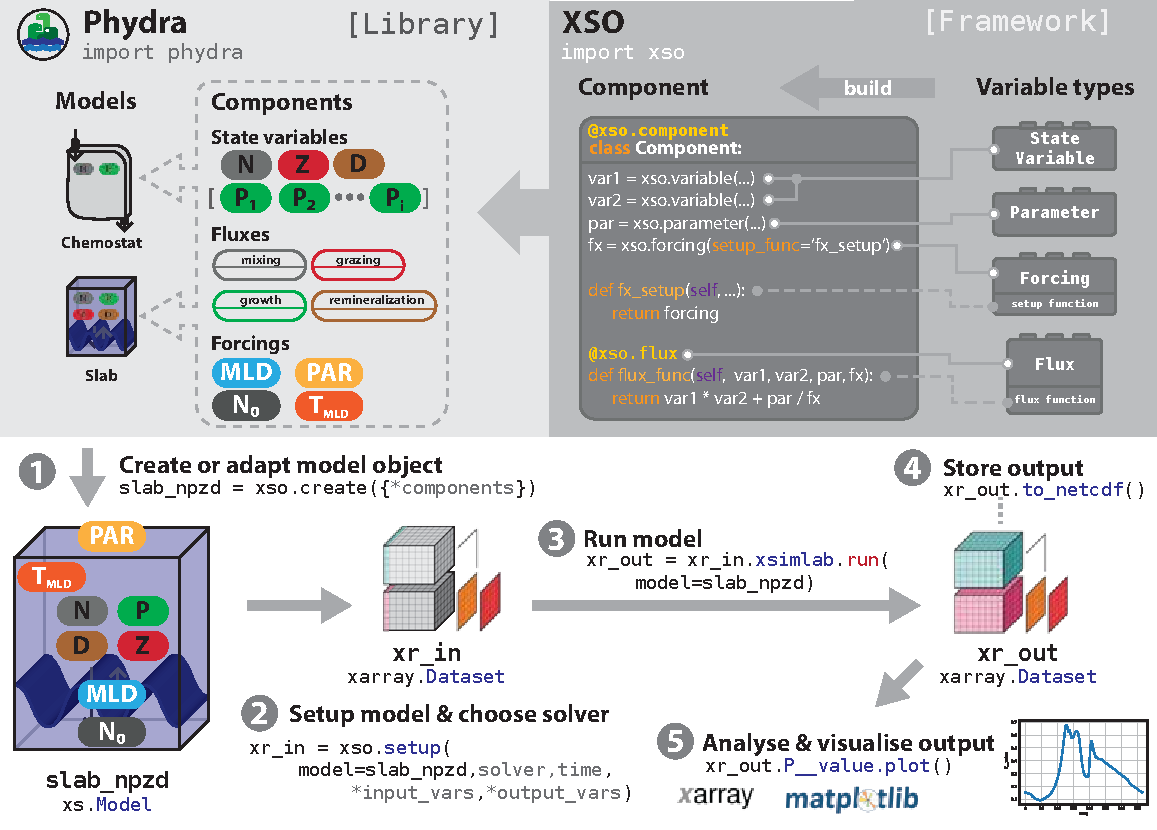
\includegraphics[width=12cm]{Figures/firstdraft_schematics/00_schematics_Package.pdf}
\caption{\textit{This is slightly outdated, and will need to be updated to represent the latest version of the workflow (once the code base is fixed).} The phydra package is embedded within the xarray-simlab framework. phydra contains a library of physical settings (1), components (i.e. state variables) (2), fluxes (3) and forcing variables (4), that can be combined and reused to create an xarray-simlab model instance. Xarray-simlab provides the functionality to define the model (5) from processes in the phydra library, supply parameters and create an xarray input (6), then run the model (7) and the resulting output is dynamically stored in another xarray, with fully labelled dimensions and containing all parameters.}
\label{Figure:phydraschematics}
\end{figure*}


Phydra is a tool-box for marine ecosystem modeling, that is freely extensible by a user to be applied to many different use cases. Our goal is to make the technical implementation of writing functions and setting up a model more accessible, so that the focus can be on creating the most appropriate model structure and parameterisation for the specific scientific hypothesis that is being investigated. 

Constructing marine ecosystem models in Phydra is by design a flexible process, but the user can follow a general workflow of assembling models from the library of processes. This workflow is visualized in Figure \ref{Figure:phydraschematics} and will be further explained below.

\subsubsection{Installing and running Phydra}
The Phydra package is available via the Python pip package manager, but we encourage using Conda as a package manager that is provided with the scientific Anaconda Python distribution.
Please follow the up-to-date instructions on the Github repository for installation of Phydra and its dependencies.

% CONDA NAME DROP
Since Python and the dependencies of Phydra are constantly developed further, we will provide instructions to install a fully compatible virtual environment with the Conda package manager separate from a users standard Python installation. For interactive coding and prototyping of models using Phydra, we recommend using the Jupyter environment that is available via Conda. For more complex and larger model runs on servers Python scripts are preferable.


\subsubsection{Model creation}

To create a Phydra model object, the desired processes defining state variables, forcings and fluxes have to be provided with their corresponding label to the \texttt{phydra.Model()} function.
The model can be assembled from the Phydra library, modifications of provided base classes or custom written processes. Multiple instances of fluxes or components can easily be added to the model, as long as the provided label differentiates them.
These labels will be the specific name of the process in this model instance. At model setup, the labels are used to reference a process and provide the appropriate parameters.

When creating a model, the xarray-simlab framework automatically checks that all references between processes are fulfilled, orders the processes in their logical order of execution and returns a Phydra model object. This model object contains all processes in the model and allows the user to view all parameters required as input at model setup. The Phydra library provides several basic model objects, that can be modified by a user through a simple interface that allows removing, modifying or adding new processes.

\subsubsection{Model setup}

A Phydra model object is itself only a collection of abstract processes. In order to fully initialize a model that can be solved, the model object needs to be supplied with a complete set of parameters.

This is done using the \texttt{phydra.create\_setup()} function. The necessary arguments to this function are the model object to be setup, all required input parameters, the time range to solve the model and the specific model output to save during runtime. The Phydra setup function is a thin wrapper around the Xarray-simlab model setup function that automatically includes the solver backend and clocks setup for the chosen solving method.

Phydra provides several options to store model output, as well as storing the value of fluxes and forcings. This allows users to specify the model output that suits the complexity of the model construct. There are processes supplied that can aggregate all state variables, Forcings or Fluxes values for output storage to simplify the process of defining output. For complex functional group models the output of each component can be stored along an individually labelled dimension, while a simple NPZD model can store the output of components along a shared dimension.

The function call returns an Xarray dataset object that contains all provided parameters as well as the initialized labelled model dimensions. This dataset can be passed with the appropriate model object to be solved in the next step, but also provides an interface to exchange parameters to easily modify an already instantiated model setup.

At model setup, the xarray-simlab framework supports batch dimensions of single or multiple parameters along which the model can be solved in parallel at runtime. This provides an efficient and intuitive interface to explore the parameter space of models.

\subsubsection{Runtime}
% -> model_instance.xsimlab.run()
% relatively straightforward, this will first initialize the model data variables according to the added processes and parameters supplied, and then start model evaluation
The model setup created in the previous step already contains the necessary parameters and labelled dataset for model runtime. All that is required of the user is to call the \texttt{xsimlab.run()} attribute and provide a model object that corresponds to the model setup. This does not have to be the same model instance used to create the setup, as long as specified parameters and output are compatible.

\textit{NOTE: Currently there is only one way to solve models in Phydra: using the GEKKO dynamic sequential solver (IMODE 7).. but there are a few options to relatively easily provide an interface for other types of solvers for future versions. Not sure if I should mention the following:}

-GEKKO provides a simple interface for steady state-simulations, and model optimisation. The models constructed with Phydra are completely compatible, simply the solver process needs to be exchanged (and for model optimisation an objective function needs to be defined additionally)

- GEKKO does as of yet not provide an adaptive step size solver like odeint, but I have created a feature request and talked to the developers. This will very likely be included in future versions.

\subsubsection{Model Diagnostics and additional functionality}

- If the option is specified at setup, the model output will include not just the state variables, but the values of all fluxes. The magnitude of the fluxes can then easily be plotted...

- Xarray-simlab provides visualisation functions, that can be used to get a structured overview over all processes in a model instance. These are not optimized for the current structure though, as most dependencies between subprocesses are handled in the solver backend, not via explicit xarray-simlab process dependencies.

- Gekko stores model equations including the names of parameters and it would be possible to add some functions that print the mathematical equations.. which would be quite helpful to build and debug a model. (possible feature)

- Model optimisation (i.e. parameter fitting) is well supported by the GEKKO backend. I will run some tests, and if it works very well, it might make sense to include it in this publication, since it is a major strong point for using Phydra.

\subsubsection{Modification and further development}

The object-oriented structure of Phydra allows users to extend certain base processes to provide the desired functionality. 

Similar to how a forcing process can easily be sub-classed to supply a different type of forcing to the environment, other processes can be easily modified to have a different function, as long as the interaction between state variables matches with the dimensions and overall structure of the components involved. 

% OPEN SOURCE CONTRIBUTION 
Phydra (like Xarray-simlab and GEKKO) is an open-source project. Contributions are welcome and in fact greatly appreciated. Users can contribute in many ways by reporting bugs, submitting feedback, contributing to the development of the code or the documentation. Please read the contributing guidelines on the Github repository for further details.

%% END OF SECTION 2
\clearpage

\textit{Note: I have already written a lot of text here, then moved it to the Appendix and started writing again. I was experimenting with ways to present model structure, and currently the most finished is Use Case 1. It should be relatively easy to implement the same type of presentation for the other use cases, once the common structure is set. For a concise and complete overview of the models, please see the appendix. Sorry for the half-baked text, it probably doesn't make sense to review it in detail. Once the model example code is fully done (within the next weeks) I should be able to write this down a lot more easily.}

 %% \ SECTION 3
\section{Use cases} \label{Section:UseCases}
% STAY AS FAR AS POSSIBLE AWAY FROM SPECIFIC PHYDRA/XARRAY_SIMLAB_ODE IMPLEMENTATION (I:E: LABELS ETC:) JUST TALK ABOUT COMPONENTS IF NECESSARY::

To showcase the utility of Phydra, we present three model use cases of varying complexity. In this section, we present simplified descriptions of model structure and mechanisms, following the model development workflow presented in Section \ref{Section:phydrapackage}.
Per use case, we first describe the generic physical environment employed. The environment collects the model components and computes common forcing fluxes. After describing the model components and what they represent, we move on to describe the fluxes that define the interactions between components. Finally, setup \& parameters for the model runtime are presented and simulation results are shown.

For a complete structure-independent mathematical description of the presented models please see Appendix 1. Additionally model and analysis code for all use cases is publicly available as documented interactive Jupyter notebooks in the Phydra repository (\url{https://github.com/ben1post/phydra/tree/master/examples}). 

\subsection{A simple chemostat model}
TEXT

\subsubsection{Description}
% really present a concise and to the point model description here, as would be in any other model publication.

\subsubsection{Implementation}
% here present the implementation as is used in phydra

\subsubsection{Results}
TEXT


\subsection{An NPZD slab model: EMPOWER}
Our second use case presents a classical NPZD model embedded in a slab-ocean physical setting. The simplified two-layer structure provides a zero-dimensional and mechanistically simple description of physical processes affecting euphotic ecosystems in the open ocean. The classical structure lends itself well as an efficient physical test-bed for more complicated ecosystem descriptions and is often used as a teaching example.

The presented model is an implementation of the elegant EMPOWER model, as presented by \citet{Anderson2015c}. 
See Figure \ref{Figure:phydraschematics_1} (a) for a schematic of the model structure and please refer to Appendix 1.1 for the full system of equations.

\subsubsection{Description}
% really present a concise and to the point model description here, as would be in any other model publication.

\subsubsection{Implementation}
% here present the implementation as is used in phydra

\subsubsection{Results}
% show model results and discuss 


\subsection{An complex size-based NPZ model: ASTroCAT}

From an attempt at describing an oceanic physical setting with a highly simplified ecosystem, we move to a simplified laboratory setting with a complex description of a size-structured ecosystem. The model structure for the second use case was adapted from \cite{Banas2011b}. See Figure \ref{Figure:phydraschematics_1} (b) for a schematic of the model structure. 

- Chemostats, a.k.a. continuous cultures, have been regularly used in exploring properties of phytoplankton! Seminal studies of Droop on nutrient uptake were performed using chemostats. \citep{Droop1968VitaminLutheri} 
- also to this day, still an interesting, very simple setting for phytoplankton models

Size is called a "master-trait" in the trait-based description of plankton ecology, allowing modellers and ecologist to describe the diverse plankton community along one continuous axis. (This is of course an oversimplification, and it takes careful consideration of the choice of allometries and often a combination of functional properties and size classes to achieve a more realistic representation of natural phytoplankton assemblages.)

See Figure \ref{Figure:phydraschematics_1} (b) for a schematic of the model structure. See Appendix 1.2 for the full system of equations.


\subsubsection{Description}
% really present a concise and to the point model description here, as would be in any other model publication.

\subsubsection{Implementation}
% here present the implementation as is used in phydra

\subsubsection{Results}
TEXT



\conclusions  %% \conclusions[modified heading if necessary]
% Place this project in the wider open science ecosystem, outlook on further developments











%% The following commands are for the statements about the availability of data sets and/or software code corresponding to the manuscript.
%% It is strongly recommended to make use of these sections in case data sets and/or software code have been part of your research the article is based on.

\codeavailability{TEXT} %% use this section when having only software code available


\dataavailability{TEXT} %% use this section when having only data sets available


\codedataavailability{TEXT} %% use this section when having data sets and software code available


\sampleavailability{TEXT} %% use this section when having geoscientific samples available


\videosupplement{TEXT} %% use this section when having video supplements available


\appendix
\section{}    %% Appendix A

\subsection{}     %% Appendix A1, A2, etc.


\noappendix       %% use this to mark the end of the appendix section. Otherwise the figures might be numbered incorrectly (e.g. 10 instead of 1).

%% Regarding figures and tables in appendices, the following two options are possible depending on your general handling of figures and tables in the manuscript environment:

%% Option 1: If you sorted all figures and tables into the sections of the text, please also sort the appendix figures and appendix tables into the respective appendix sections.
%% They will be correctly named automatically.

%% Option 2: If you put all figures after the reference list, please insert appendix tables and figures after the normal tables and figures.
%% To rename them correctly to A1, A2, etc., please add the following commands in front of them:

\appendixfigures  %% needs to be added in front of appendix figures

\appendixtables   %% needs to be added in front of appendix tables

%% Please add \clearpage between each table and/or figure. Further guidelines on figures and tables can be found below.



\authorcontribution{TEXT} %% this section is mandatory

\competinginterests{TEXT} %% this section is mandatory even if you declare that no competing interests are present

\disclaimer{TEXT} %% optional section

\begin{acknowledgements}
TEXT
\end{acknowledgements}




%% REFERENCES

%% The reference list is compiled as follows:

\begin{thebibliography}{}

\bibitem[AUTHOR(YEAR)]{LABEL1}
REFERENCE 1

\bibitem[AUTHOR(YEAR)]{LABEL2}
REFERENCE 2

\end{thebibliography}

%% Since the Copernicus LaTeX package includes the BibTeX style file copernicus.bst,
%% authors experienced with BibTeX only have to include the following two lines:
%%
%% \bibliographystyle{copernicus}
%% \bibliography{example.bib}
%%
%% URLs and DOIs can be entered in your BibTeX file as:
%%
%% URL = {http://www.xyz.org/~jones/idx_g.htm}
%% DOI = {10.5194/xyz}


%% LITERATURE CITATIONS
%%
%% command                        & example result
%% \citet{jones90}|               & Jones et al. (1990)
%% \citep{jones90}|               & (Jones et al., 1990)
%% \citep{jones90,jones93}|       & (Jones et al., 1990, 1993)
%% \citep[p.~32]{jones90}|        & (Jones et al., 1990, p.~32)
%% \citep[e.g.,][]{jones90}|      & (e.g., Jones et al., 1990)
%% \citep[e.g.,][p.~32]{jones90}| & (e.g., Jones et al., 1990, p.~32)
%% \citeauthor{jones90}|          & Jones et al.
%% \citeyear{jones90}|            & 1990



%% FIGURES

%% When figures and tables are placed at the end of the MS (article in one-column style), please add \clearpage
%% between bibliography and first table and/or figure as well as between each table and/or figure.

% The figure files should be labelled correctly with Arabic numerals (e.g. fig01.jpg, fig02.png).


%% ONE-COLUMN FIGURES

%%f
%\begin{figure}[t]
%\includegraphics[width=8.3cm]{FILE NAME}
%\caption{TEXT}
%\end{figure}
%
%%% TWO-COLUMN FIGURES
%
%%f
%\begin{figure*}[t]
%\includegraphics[width=12cm]{FILE NAME}
%\caption{TEXT}
%\end{figure*}
%
%
%%% TABLES
%%%
%%% The different columns must be seperated with a & command and should
%%% end with \\ to identify the column brake.
%
%%% ONE-COLUMN TABLE
%
%%t
%\begin{table}[t]
%\caption{TEXT}
%\begin{tabular}{column = lcr}
%\tophline
%
%\middlehline
%
%\bottomhline
%\end{tabular}
%\belowtable{} % Table Footnotes
%\end{table}
%
%%% TWO-COLUMN TABLE
%
%%t
%\begin{table*}[t]
%\caption{TEXT}
%\begin{tabular}{column = lcr}
%\tophline
%
%\middlehline
%
%\bottomhline
%\end{tabular}
%\belowtable{} % Table Footnotes
%\end{table*}
%
%%% LANDSCAPE TABLE
%
%%t
%\begin{sidewaystable*}[t]
%\caption{TEXT}
%\begin{tabular}{column = lcr}
%\tophline
%
%\middlehline
%
%\bottomhline
%\end{tabular}
%\belowtable{} % Table Footnotes
%\end{sidewaystable*}
%
%
%%% MATHEMATICAL EXPRESSIONS
%
%%% All papers typeset by Copernicus Publications follow the math typesetting regulations
%%% given by the IUPAC Green Book (IUPAC: Quantities, Units and Symbols in Physical Chemistry,
%%% 2nd Edn., Blackwell Science, available at: http://old.iupac.org/publications/books/gbook/green_book_2ed.pdf, 1993).
%%%
%%% Physical quantities/variables are typeset in italic font (t for time, T for Temperature)
%%% Indices which are not defined are typeset in italic font (x, y, z, a, b, c)
%%% Items/objects which are defined are typeset in roman font (Car A, Car B)
%%% Descriptions/specifications which are defined by itself are typeset in roman font (abs, rel, ref, tot, net, ice)
%%% Abbreviations from 2 letters are typeset in roman font (RH, LAI)
%%% Vectors are identified in bold italic font using \vec{x}
%%% Matrices are identified in bold roman font
%%% Multiplication signs are typeset using the LaTeX commands \times (for vector products, grids, and exponential notations) or \cdot
%%% The character * should not be applied as mutliplication sign
%
%
%%% EQUATIONS
%
%%% Single-row equation
%
%\begin{equation}
%
%\end{equation}
%
%%% Multiline equation
%
%\begin{align}
%& 3 + 5 = 8\\
%& 3 + 5 = 8\\
%& 3 + 5 = 8
%\end{align}
%
%
%%% MATRICES
%
%\begin{matrix}
%x & y & z\\
%x & y & z\\
%x & y & z\\
%\end{matrix}
%
%
%%% ALGORITHM
%
%\begin{algorithm}
%\caption{...}
%\label{a1}
%\begin{algorithmic}
%...
%\end{algorithmic}
%\end{algorithm}
%
%
%%% CHEMICAL FORMULAS AND REACTIONS
%
%%% For formulas embedded in the text, please use \chem{}
%
%%% The reaction environment creates labels including the letter R, i.e. (R1), (R2), etc.
%
%\begin{reaction}
%%% \rightarrow should be used for normal (one-way) chemical reactions
%%% \rightleftharpoons should be used for equilibria
%%% \leftrightarrow should be used for resonance structures
%\end{reaction}
%
%
%%% PHYSICAL UNITS
%%%
%%% Please use \unit{} and apply the exponential notation


\end{document}
